\section{Entrenamiento y Evaluación de Modelos}\label{sec:entrenamiento}

\subsection{Configuración experimental}

\subsubsection{Preprocesamiento, codificación e imputación}\label{sec:prep}
Las once predictoras son categóricas y se codificaron de tres maneras, resumidas en el Cuadro~\ref{tab:codif_def}. En la codificación A ninguna variable se imputa: el faltante se convierte en una categoría más, ``no reportado'', y todas pasan a \textit{one-hot}; así, sexo genera 2 columnas, cada binaria de estilo de vida (actividad física, alcohol, frutas y vegetales) 3 (sí, no, no reportado), raza/etnia 6 y fumador 5. En las codificaciones B y C, edad, educación, ingreso e IMC se tratan como enteros estandarizados porque tienen un orden natural, y las nominales siguen en \textit{one-hot}; los faltantes se imputan con la moda global de cada variable. Se usó la moda y no la mediana porque las variables son categóricas, y se descartó imputar con la moda de cada clase porque al predecir la clase es desconocida y usarla en el ajuste filtraría la etiqueta. C agrega además un indicador binario de faltante por variable.

\begin{table}[!t]
\centering
\caption{Codificaciones evaluadas y número de columnas que produce cada una}
\label{tab:codif_def}
\footnotesize
\setlength{\tabcolsep}{2.5pt}
\begin{tabular}{@{}L{2.4cm}L{2.6cm}L{3.5cm}@{}}
\toprule
\textbf{Variables} & \textbf{A: \textit{one-hot} + no reportado} & \textbf{B / C: ordinal + moda (C: + indicador)} \\
\midrule
Sexo & 2 columnas & \textit{One-hot}, 2 columnas \\
Actividad física, alcohol, frutas, vegetales & 3 columnas c/u & \textit{One-hot}, 2 columnas c/u \\
Raza/etnia, fumador & 6 y 5 columnas & \textit{One-hot}, 5 y 4 columnas \\
Edad, educación, ingreso, IMC & 14, 5, 8 y 5 columnas & 1 columna estandarizada c/u \\
\midrule
Total & 57 & B: 23; C: 39 \\
\bottomrule
\end{tabular}
\end{table}

La moda, la estandarización y las categorías del \textit{one-hot} se ajustan dentro de un \textit{pipeline}, de modo que en cada pliegue de validación se calculan solo con los datos de entrenamiento de ese pliegue, y en el modelo final solo con el conjunto de entrenamiento. Antes de elegir se revisó, también solo con entrenamiento, si no responder se asocia con la diabetes. La prevalencia cambia de forma significativa ($\chi^2$, $p<0{,}01$) entre quienes respondieron y quienes no en edad, educación, IMC, actividad física, fumador y alcohol; en actividad física, por ejemplo, pasa de 15,11\% a 21,15\%, y en alcohol de 15,31\% a 13,11\%. En raza/etnia, ingreso, frutas y vegetales no hay diferencia ($p>0{,}05$). Es decir, en varias variables el hecho de no responder sí trae información, y por eso A y C la conservan como predictor.

El orden de las ordinales se revisó de forma directa (Fig.~\ref{fig:prop}): con la regresión logística en \textit{one-hot}, el coeficiente de cada categoría muestra cuánto cambia el log-odds frente a la primera. Si el orden fuera proporcional, los puntos caerían sobre una recta. IMC (R$^2=0{,}98$) e ingreso (0,96) se acercan bastante, pero la edad no: el riesgo sube rápido hasta los 55--59 años, después crece mucho más despacio y baja en el grupo de 80 años o más, con pasos entre categorías que van de $-$0,16 a 0,49. En educación, los niveles 2 y 3 prácticamente no se distinguen. Por eso no se impuso una codificación, sino que cada modelo usa A salvo que B o C la superen en AUC de validación con diferencia significativa (prueba $t$ pareada sobre los mismos pliegues, $p<0{,}05$).

\begin{figure*}[!t]
\centering
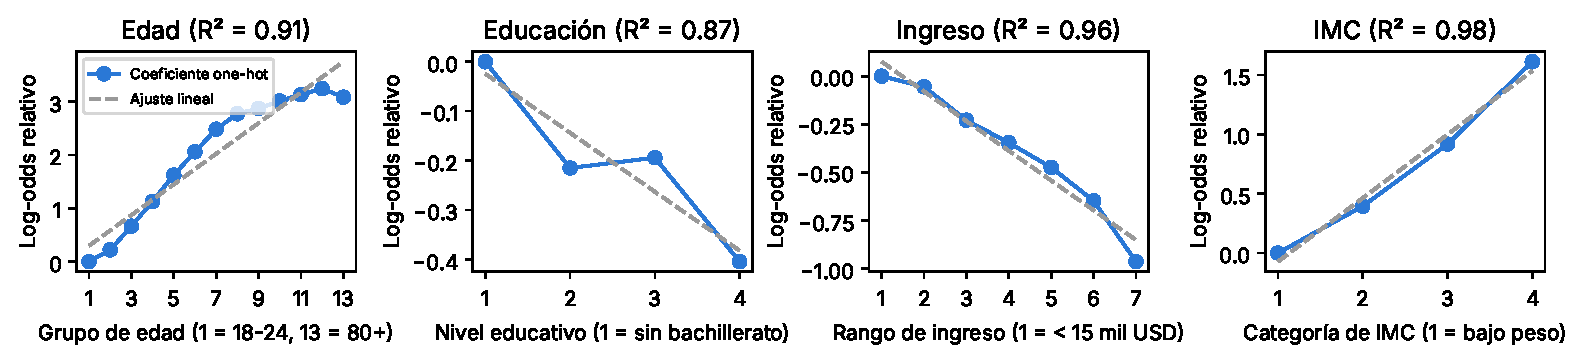
\includegraphics[width=0.94\textwidth]{proporcionalidad_ordinales.pdf}
\caption{Coeficientes de la regresión logística con codificación \textit{one-hot} para cada categoría de las variables ordinales, relativos a la primera categoría (línea continua), y su ajuste lineal (línea discontinua). Un ajuste lineal perfecto indicaría que tratar la variable como entero no pierde información.}
\label{fig:prop}
\end{figure*}

\subsubsection{Metodología de validación}
Los 342.539 registros se dividieron de forma estratificada en entrenamiento (80\%, 274.031) y prueba (20\%, 68.508); la prueba se apartó desde el inicio y se usó una sola vez. Atendiendo al costo computacional, la búsqueda de hiperparámetros se hizo con validación cruzada estratificada de 5 pliegues sobre una submuestra estratificada de 20.000 registros de entrenamiento, que conserva el 15,13\% de positivos: la SVM con kernel RBF escala de forma cuadrática con el número de muestras y tardó más de 15 minutos solo en esa malla. Cada métrica se reporta como la media de los 5 pliegues con su intervalo de confianza (IC) del 95\%, $\bar{x} \pm t_{0{,}975;\,4}\, s/\sqrt{5}$. Con los mejores hiperparámetros, cada modelo se reajustó con todo el entrenamiento y se evaluó en prueba, salvo la SVM, que se reajustó con una submuestra estratificada de 40.000 registros. En prueba, los IC se estimaron con 1.000 remuestreos \textit{bootstrap}.

\subsubsection{Manejo del desbalance}
Toda corrección del desbalance va dentro del \textit{pipeline}, así que se aplica solo a los pliegues de entrenamiento; validación y prueba conservan la proporción real de clases. La regresión logística, el bosque aleatorio y la SVM usan ponderación de clases inversamente proporcional a su frecuencia. KNN y el perceptrón multicapa no admiten ponderación en \textit{scikit-learn} y usan submuestreo aleatorio de la clase mayoritaria. El Cuadro~\ref{tab:balanceo} sustenta esta elección.

\subsubsection{Modelos e hiperparámetros}
Se compararon cinco modelos, uno por familia: regresión logística con regularización L2 (paramétrico), $k$ vecinos más cercanos (no paramétrico), bosque aleatorio (ensamble de árboles), perceptrón multicapa (red neuronal; ReLU, Adam y parada temprana) y SVM con kernel RBF. El Cuadro~\ref{tab:malla} presenta las mallas: 69 combinaciones, cada una evaluada en los 5 pliegues.

\begin{table}[!t]
\centering
\caption{Malla de hiperparámetros de cada modelo y valor elegido por mayor AUC de validación}
\label{tab:malla}
\footnotesize
\setlength{\tabcolsep}{3pt}
\begin{tabular}{@{}p{1.75cm}p{1.9cm}p{3.25cm}p{1.1cm}@{}}
\toprule
\textbf{Modelo} & \textbf{Parámetro} & \textbf{Valores} & \textbf{Elegido} \\
\midrule
Reg. logística & $C$ & $10^{-3}, 10^{-2}, \ldots, 10^{2}$ & 1 \\
\addlinespace
KNN & Vecinos $k$ & 5, 15, 31, 51, 101, 201, 401 & 401 \\
 & Pesos & uniforme, distancia & uniforme \\
\addlinespace
Bosque & N.º de árboles & 100, 300 & 100 \\
aleatorio & Prof. máxima & 4, 8, 12, sin límite & 12 \\
 & Mín. por hoja & 1, 10, 50 & 10 \\
\addlinespace
Red neuronal & Capas ocultas & (16), (64), (32, 16), (64, 32) & (16) \\
(MLP) & $\alpha$ (L2) & $10^{-4}, 10^{-2}, 10^{-1}, 1$ & $10^{-4}$ \\
\addlinespace
SVM (RBF) & $C$ & 0,1; 1; 10 & 1 \\
 & $\gamma$ & $10^{-3}, 10^{-2}, 10^{-1}$ & $10^{-2}$ \\
\bottomrule
\end{tabular}
\end{table}

\subsubsection{Métricas de desempeño}
Los hiperparámetros se eligen por el área bajo la curva ROC (AUC), que no depende del umbral de decisión ni de la proporción de clases. La sensibilidad es la métrica de monitoreo clave: en tamizaje, un falso negativo es una persona con diabetes que no se remite a evaluación, mientras que un falso positivo solo implica un examen adicional. Se reportan además la especificidad, que mide el costo en falsas alarmas, la precisión y el F1. La exactitud no se usa como criterio, porque un modelo que siempre predice ``no'' llegaría a 84,87\% sin detectar un solo caso.

\subsection{Resultados del entrenamiento de modelos}

\subsubsection{Codificación y desbalance}
Según el Cuadro~\ref{tab:codificacion}, la mejor codificación depende del modelo. La regresión logística pierde AUC al tratar las ordinales como enteros (0,66 puntos porcentuales, pp, con B; $p<0{,}01$), lo que coincide con la falta de proporcionalidad de la edad (Fig.~\ref{fig:prop}). Los modelos basados en distancias, en cambio, mejoran: KNN gana 4,24 pp con B ($p<0{,}01$) y la SVM 1,44 pp con C ($p<0{,}01$), porque así dos grupos de edad contiguos quedan más cerca que dos lejanos, mientras que en \textit{one-hot} todas las categorías están a la misma distancia. En el bosque aleatorio y la red neuronal las diferencias no son significativas y se conserva A.

\begin{table}[!t]
\centering
\caption{AUC de validación (media $\pm$ IC 95\%) según la codificación, y mayor diferencia frente a A en puntos porcentuales (pp). En negrita, la codificación adoptada}
\label{tab:codificacion}
\footnotesize
\setlength{\tabcolsep}{3pt}
\begin{tabular}{@{}lcccc@{}}
\toprule
\textbf{Modelo} & \textbf{A} & \textbf{B} & \textbf{C} & \textbf{Dif. (valor $p$)} \\
\midrule
Reg. logística & \textbf{0,76\,$\pm$\,0,01} & 0,75\,$\pm$\,0,01 & 0,75\,$\pm$\,0,01 & B: $-$0,66 (\textless 0,01) \\
KNN & 0,70\,$\pm$\,0,01 & \textbf{0,74\,$\pm$\,0,01} & 0,73\,$\pm$\,0,01 & B: +4,24 (\textless 0,01) \\
Bosque aleatorio & \textbf{0,75\,$\pm$\,0,01} & 0,75\,$\pm$\,0,01 & 0,75\,$\pm$\,0,01 & C: +0,35 (0,13) \\
Red neuronal & \textbf{0,75\,$\pm$\,0,01} & 0,75\,$\pm$\,0,01 & 0,75\,$\pm$\,0,02 & B: +0,06 (0,80) \\
SVM (RBF) & 0,73\,$\pm$\,0,01 & 0,75\,$\pm$\,0,01 & \textbf{0,75\,$\pm$\,0,01} & C: +1,44 (\textless 0,01) \\
\bottomrule
\end{tabular}
\end{table}

Sin corrección del desbalance (Cuadro~\ref{tab:balanceo}) los modelos conservan el AUC, pero casi no detectan positivos: la sensibilidad de la regresión logística cae a 0,04 y la del bosque a 0,00. SMOTE no mejora frente a la ponderación de clases: en la regresión logística baja el AUC 0,38 pp ($p<0{,}01$) y la sensibilidad 1,02 pp ($p=0{,}03$), y en el bosque la sensibilidad cae 29,87 pp ($p<0{,}01$). SMOTEN, la variante para variables categóricas, es la peor opción, con pérdidas de AUC cercanas a 4 pp. El submuestreo aleatorio rinde como la ponderación, lo que respalda su uso en KNN y la red neuronal.

\begin{table}[!t]
\centering
\caption{Desempeño en validación (media $\pm$ IC 95\%) según la estrategia para el desbalance de clases}
\label{tab:balanceo}
\footnotesize
\setlength{\tabcolsep}{3pt}
\begin{tabular}{@{}lccc@{}}
\toprule
\textbf{Estrategia} & \textbf{AUC} & \textbf{Sensibilidad} & \textbf{Especificidad} \\
\midrule
\multicolumn{4}{@{}l}{\textit{Regresión logística}} \\
\quad Sin corrección & 0,76\,$\pm$\,0,01 & 0,04\,$\pm$\,0,01 & 0,99\,$\pm$\,0,00 \\
\quad Ponderación de clases & 0,76\,$\pm$\,0,01 & 0,75\,$\pm$\,0,01 & 0,64\,$\pm$\,0,01 \\
\quad SMOTE & 0,75\,$\pm$\,0,01 & 0,74\,$\pm$\,0,02 & 0,64\,$\pm$\,0,01 \\
\quad SMOTEN & 0,72\,$\pm$\,0,01 & 0,64\,$\pm$\,0,02 & 0,67\,$\pm$\,0,00 \\
\quad Submuestreo aleatorio & 0,76\,$\pm$\,0,01 & 0,74\,$\pm$\,0,01 & 0,64\,$\pm$\,0,02 \\
\multicolumn{4}{@{}l}{\textit{Bosque aleatorio}} \\
\quad Sin corrección & 0,74\,$\pm$\,0,01 & 0,00\,$\pm$\,0,00 & 1,00\,$\pm$\,0,00 \\
\quad Ponderación de clases & 0,75\,$\pm$\,0,01 & 0,72\,$\pm$\,0,02 & 0,65\,$\pm$\,0,02 \\
\quad SMOTE & 0,74\,$\pm$\,0,01 & 0,42\,$\pm$\,0,03 & 0,84\,$\pm$\,0,01 \\
\quad SMOTEN & 0,71\,$\pm$\,0,01 & 0,53\,$\pm$\,0,02 & 0,75\,$\pm$\,0,01 \\
\quad Submuestreo aleatorio & 0,74\,$\pm$\,0,01 & 0,72\,$\pm$\,0,01 & 0,63\,$\pm$\,0,02 \\
\bottomrule
\end{tabular}
\end{table}

\subsubsection{Efecto de los hiperparámetros}
La Fig.~\ref{fig:hiper} muestra el AUC de entrenamiento y validación a lo largo de cada malla. En la regresión logística (a) solo la regularización más fuerte ($C=10^{-3}$) produce subajuste; desde $C=0{,}1$ el modelo ya no cambia. En KNN (b) el AUC de validación crece con $k$ hasta estabilizarse alrededor de $k=200$, y la ponderación por distancia sobreajusta: con datos categóricos abundan los vecinos a distancia cero, que reciben peso infinito. El bosque aleatorio (c) memoriza los datos cuando los árboles crecen sin límite y con hojas de una muestra, y se corrige al limitar la profundidad o exigir al menos 10 muestras por hoja; pasar de 100 a 300 árboles no cambia nada. La red neuronal (d) es poco sensible a la arquitectura y a $\alpha$, pues todas las combinaciones quedan dentro del IC de las demás. En la SVM (e), $\gamma=0{,}1$ con $C=10$ sobreajusta (AUC de 0,88 en entrenamiento y 0,71 en validación), mientras que $\gamma \leq 10^{-2}$ da fronteras suaves que generalizan mejor.

\begin{figure*}[!t]
\centering
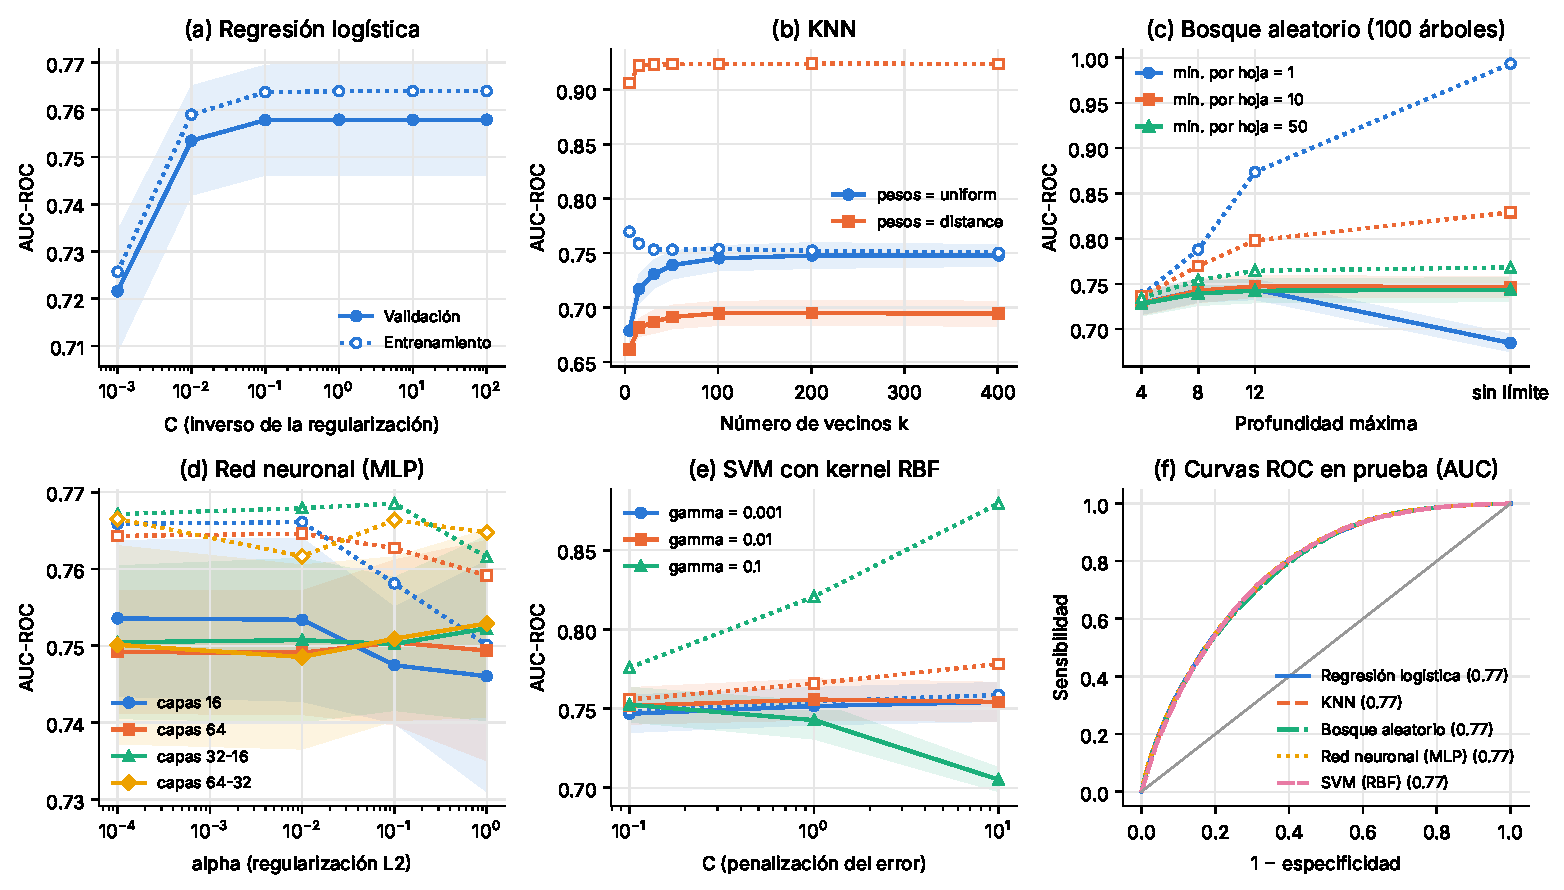
\includegraphics[width=0.9\textwidth]{hiperparametros_y_roc.pdf}
\caption{Efecto de los hiperparámetros sobre el AUC-ROC en la validación cruzada de 5 pliegues: (a) regresión logística, (b) KNN, (c) bosque aleatorio, (d) red neuronal y (e) SVM. La línea continua es la media de validación y la banda su IC del 95\%; la línea punteada es la media de entrenamiento. (f) Curvas ROC de los cinco modelos finales en el conjunto de prueba, con su AUC entre paréntesis.}
\label{fig:hiper}
\end{figure*}

\subsubsection{Desempeño final}
El Cuadro~\ref{tab:resultados} resume cada modelo con sus mejores hiperparámetros. En validación el AUC va de 0,75 a 0,76, con intervalos que se traslapan, y en prueba los cinco llegan a 0,77: ninguna familia es superior a las demás, y las curvas ROC son prácticamente indistinguibles (Fig.~\ref{fig:hiper}f). Esto sugiere que el techo lo ponen las once variables de encuesta y no la complejidad del modelo. El valor queda dentro del rango de 0,72 a 0,79 que reportan Xie et al. \cite{xie2019} con la misma encuesta. El AUC de prueba es algo mayor que el de validación porque los modelos finales se ajustan con muchos más datos (274.031 registros frente a 16.000 por pliegue). Solo el bosque aleatorio muestra una brecha apreciable entre entrenamiento y validación (0,80 frente a 0,75), que no se traduce en un peor resultado en prueba.

\begin{table*}[!t]
\centering
\caption{Desempeño de los cinco modelos con sus mejores hiperparámetros. Entrenamiento (Ent.) y validación (Val.): media $\pm$ IC 95\% sobre los 5 pliegues. Prueba: evaluación única; el AUC y la sensibilidad incluyen su IC 95\% por \textit{bootstrap}}
\label{tab:resultados}
\footnotesize
\setlength{\tabcolsep}{3.3pt}
\begin{tabular}{@{}lcccccccccc@{}}
\toprule
 & \multicolumn{3}{c}{\textbf{AUC-ROC}} & \multicolumn{3}{c}{\textbf{Sensibilidad}} & \multicolumn{2}{c}{\textbf{Especificidad}} & \multicolumn{2}{c}{\textbf{F1}} \\
\cmidrule(lr){2-4} \cmidrule(lr){5-7} \cmidrule(lr){8-9} \cmidrule(l){10-11}
\textbf{Modelo} & Ent. & Val. & Prueba & Ent. & Val. & Prueba & Val. & Prueba & Val. & Prueba \\
\midrule
Regresión logística & 0,76\,$\pm$\,0,00 & 0,76\,$\pm$\,0,01 & 0,77 [0,76; 0,77] & 0,76\,$\pm$\,0,01 & 0,75\,$\pm$\,0,01 & 0,75 [0,74; 0,76] & 0,64\,$\pm$\,0,01 & 0,65 & 0,40\,$\pm$\,0,01 & 0,40 \\
KNN & 0,75\,$\pm$\,0,00 & 0,75\,$\pm$\,0,01 & 0,77 [0,76; 0,77] & 0,74\,$\pm$\,0,01 & 0,74\,$\pm$\,0,01 & 0,77 [0,76; 0,78] & 0,63\,$\pm$\,0,02 & 0,63 & 0,39\,$\pm$\,0,01 & 0,40 \\
Bosque aleatorio & 0,80\,$\pm$\,0,00 & 0,75\,$\pm$\,0,01 & 0,77 [0,76; 0,77] & 0,78\,$\pm$\,0,01 & 0,72\,$\pm$\,0,02 & 0,74 [0,73; 0,75] & 0,65\,$\pm$\,0,01 & 0,65 & 0,39\,$\pm$\,0,01 & 0,40 \\
Red neuronal (MLP) & 0,77\,$\pm$\,0,00 & 0,75\,$\pm$\,0,01 & 0,77 [0,77; 0,78] & 0,76\,$\pm$\,0,02 & 0,74\,$\pm$\,0,03 & 0,77 [0,76; 0,78] & 0,64\,$\pm$\,0,02 & 0,64 & 0,39\,$\pm$\,0,01 & 0,40 \\
SVM (RBF) & 0,77\,$\pm$\,0,00 & 0,76\,$\pm$\,0,01 & 0,77 [0,76; 0,77] & 0,79\,$\pm$\,0,00 & 0,78\,$\pm$\,0,01 & 0,80 [0,80; 0,81] & 0,61\,$\pm$\,0,01 & 0,60 & 0,39\,$\pm$\,0,01 & 0,40 \\
\bottomrule
\end{tabular}
\end{table*}

En la métrica clave hay más diferencia. La Fig.~\ref{fig:confusion} presenta las matrices de confusión en prueba normalizadas por la clase real, de modo que la diagonal es directamente la sensibilidad y la especificidad. La SVM detecta el 80\% de las personas con diabetes, contra 74\% a 77\% de los demás modelos, a cambio de la especificidad más baja (0,60). Todos superan con amplitud el 51,6\% que obtuvieron Xie et al. \cite{xie2019}. El costo común es una precisión de 0,26 a 0,28: cerca de una de cada cuatro alertas corresponde a un caso real, algo esperable con 15\% de prevalencia y aceptable para un tamizaje cuyo siguiente paso es un examen de bajo costo.

\begin{figure*}[!t]
\centering
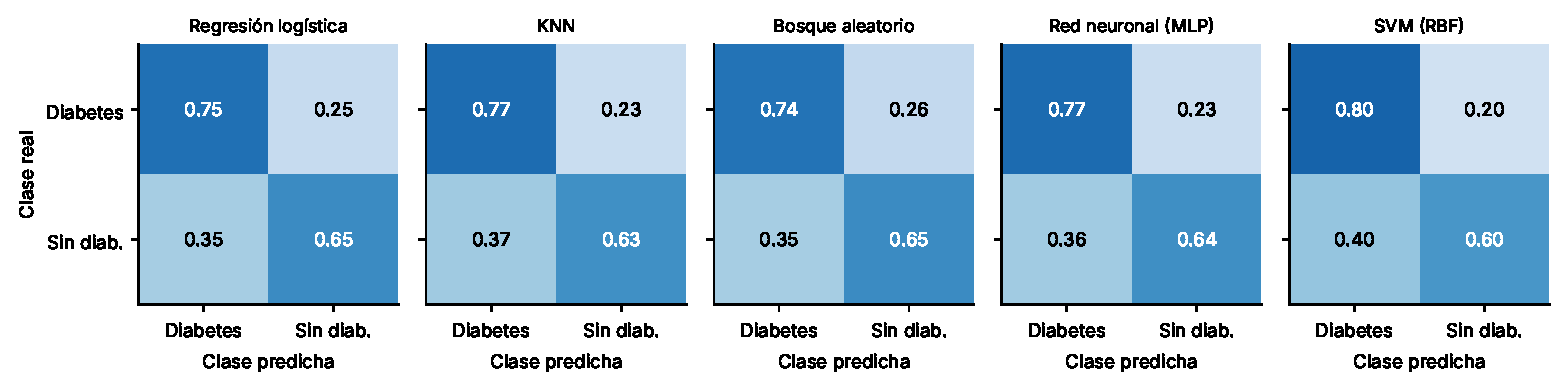
\includegraphics[width=0.92\textwidth]{matrices_confusion_normalizadas.pdf}
\caption{Matrices de confusión en el conjunto de prueba (68.508 registros), normalizadas por fila: cada celda es la fracción de la clase real que el modelo asigna a cada clase predicha.}
\label{fig:confusion}
\end{figure*}

Por último, se evaluó \texttt{LinearSVC}, que escala casi linealmente con el número de muestras. Con la codificación C su AUC de validación es 0,75\,$\pm$\,0,01 para cualquier $C$ entre 0,01 y 1, y ajustado con los 274.031 registros de entrenamiento en 1,3~s llega en prueba a un AUC de 0,76, sensibilidad de 0,73 y especificidad de 0,66. La SVM RBF, ajustada con 40.000 registros, tarda unos 5 minutos pero alcanza 0,77 de AUC y 7 puntos más de sensibilidad. Como la sensibilidad es la prioridad, se conservó el kernel RBF y se controló su costo con submuestras.

Los dos modelos con mayor AUC medio de validación, la regresión logística y la SVM (ambos 0,76), pasan a la fase de reducción de dimensión. La red neuronal queda muy cerca y la diferencia no es significativa, pero la SVM tiene además la mejor sensibilidad, y las dos elegidas representan enfoques distintos: una frontera lineal sobre variables \textit{one-hot} y una frontera no lineal sobre variables ordinales.

